\subsection{Case04 - Layer 3 forwarding}
\label{xdp_ether_case04}

En este caso de uso se explorará como realizar forwarding de paquetes. En este punto, ya se ha revisado cómo filtrar por las cabeceras de los paquetes, analizarlos y establecer una lógica asociada a ese filtrado con los códigos de retorno \gls{xdp}. Una acción adicional a realizar con los paquetes será el forwarding. En \gls{xdp} vendrá implementado por códigos de retorno y por \textit{helpers} \gls{bpf} porque, como ya comentábamos en el case02 (\ref{xdp_ether_case02}), \gls{xdp} se termina traduciendo en \gls{bpf} (e\gls{bpf}), por lo que ciertas funciones, no todas, para trabajar con \gls{bpf} están disponibles a la hora de trabajar con \gls{xdp}.\\
\par

A lo largo de este caso de uso, se han explorado las distintas maneras para lograr el forwarding con \gls{xdp}. Se ha ido desde la manera más simple a la manera más robusta y, a su vez, compleja. Para que no haya diferencias entre las distintas formas de realizar el forwarding, se ha creado un mismo escenario donde se explorarán estas vías sin que existan diferencias inducidas por este. En el caso de uso anterior ya se estaba haciendo un forwarding, ya que, con el código \texttt{XDP\_TX} se realiza un forwarding hacia la interfaz por la cual se recibió dicho paquete. Pero, ¿cómo se hace un forwarding hacia otras interfaces? Leyendo la \textit{man-page} de los \textit{helpers} \gls{bpf} se han encontrado las funciones \texttt{bpf\_redirect()}, \texttt{bpf\_redirect\_map()}, las cuales, leyendo su descripción, serán la vía utilizada para abordar esta necesidad.

\begin{lstlisting}[language=C, style=C-color, caption={Helper BPF para realizar Forwarding - Case04},label=code:case04_xdp_ether_kernprog1]
    int bpf_redirect(u32 ifindex, u64 flags);

    int bpf_redirect_map(struct bpf_map *map, u32 key, u64 flags);
\end{lstlisting}


\vspace{0.5cm}
\textbf{Compilación}\\
\par

Para compilar el programa \gls{xdp} se ha dejado un Makefile preparado en este directorio al igual que en el case03 (\ref{xdp_ether_case03}), por lo que para compilarlo únicamente hay que seguir las indicaciones del bloque \ref{code:case04_xdp_ether_compilacion}.

\begin{lstlisting}[language= bash, style=Consola, caption={Compilación programa XDP - Case04},label=code:case04_xdp_ether_compilacion]
    # En caso de no haber entrado en el directorio asignado del caso de uso
    cd TFG/src/use_cases/xdp/case04
    
    # Hacemos uso del Makefile suministrado 
    sudo make
\end{lstlisting}
\vspace{0.5cm}

Podrá encontrar más información sobre el proceso de compilación de los programas \gls{xdp} en el case02 (\ref{xdp_ether_case02}).


\vspace{0.7cm}
\textbf{Puesta en marcha del escenario}\\
\par
Para comprobar el funcionamiento de los programas \gls{xdp} se hará uso de las \textit{Network Namespace} (más información en la sección \ref{namespaces}). Como ya se comentaba, para que no suponga una barrera de entrada el concepto de las \textit{Network Namespace}, se ha dejado escrito un script para levantar el escenario, y para su posterior limpieza. Es importante señalar que el script debe ser lanzado con permisos de root. Para levantar el escenario debemos ejecutar dicho script como se indica en el bloque \ref{code:case03_xdp_ether_escenario}. Para limpiar la máquina del escenario recreado anteriormente, se puede correr el mismo script indicándole ahora el parámetro \texttt{-c} (\textit{Clean}). En el peor de los casos, y si se cree que la limpieza se no se ha realizado de manera satisfactoria, se puede llevar a cabo un reinicio de la máquina consiguiendo así que todos los entes no persistentes (\gls{veth}, netns..) desaparezcan del equipo.

\begin{lstlisting}[language= bash, style=Consola, caption={Puesta en marcha del escenario - Case04},label=code:case04_xdp_ether_escenario]
    # Para levantar el escenario (Importante hacerlo con permisos de super usuario)
    sudo ./runenv.sh -i
    
    
    # Una vez finalizado la comprobación del caso de uso, limpiaremos nuestra maquina:
    sudo ./runenv.sh -c
\end{lstlisting}
\vspace{0.5cm}

%%%%%%%%%%%%%%%%%%%%%%%%%%%%%%%%%%%%%%%%%%%%%%%%%%%%%%%%%%%%%%%%%%%%%%%%%%%%%%%%%%%%

\subsubsection{Hardcoded forwarding}
\label{xdp_ether_case04_hard}

La primera forma de implementación del forwarding es lo que denominaremos como Hardcoded forwarding, dado que es necesario hardcodear\footnote{Hardcodear: perder flexibilidad y/o prolijidad dejando valores y/o comportamientos fijos en el código del programa.} información de forwarding en el propio programa \gls{xdp}. El escenario levantado se puede apreciar en la figura \ref{fig:case04_xdp_ether_scenario1}, está compuesto de dos \textit{Network Namespace} (\texttt{uno} y \texttt{dos}), y de dos pares de \gls{veth}s (\texttt{veth0} -- \texttt{uno} y \texttt{veth0} -- \texttt{dos}) las cuales se utilizarán para comunicar las dos \textit{Network Namespaces} entre sí, a través del la \textit{Network Namespace} por defecto. En este caso el forwarding lo haremos desde la interfaz \texttt{dos} hacia la interfaz \texttt{uno}.


% figura escenario
\begin{figure}[ht]
    \centering
    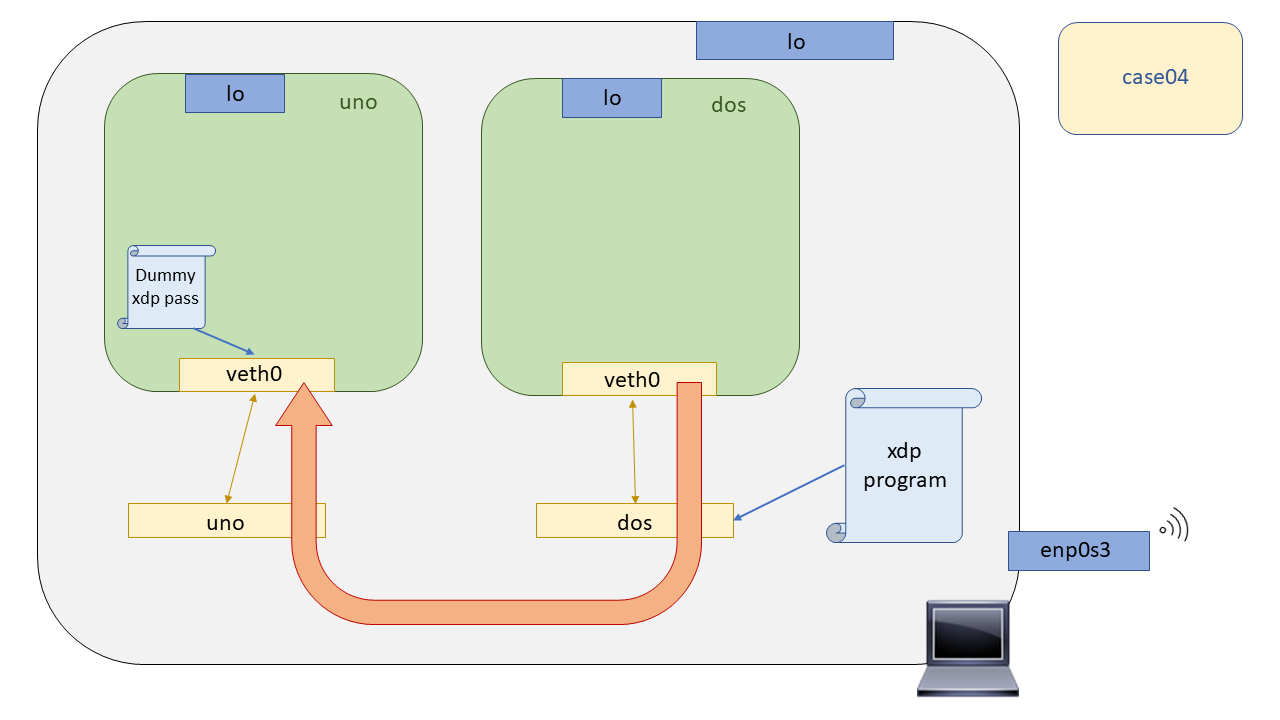
\includegraphics[width=16cm]{archivos/img/dev/xdp/case04/scenario_01.png}
    \caption{Escenario cableado Hardcoded forwarding del Case04 - XDP}
    \label{fig:case04_xdp_ether_scenario1}
\end{figure}


\vspace{0.5cm}
\textbf{Carga del programa XDP}\\
\par

Antes de realizar la carga del programa se deben obtener \textbf{dos datos}, la \textit{ifindex} de la interfaz uno a la cual se van a mandar los paquetes generados desde el interior de la \textit{Network Namespace} \texttt{dos}, y la MAC de la interfaz interna de la \textit{Network Namespace} \texttt{uno}, ya que será necesario que los paquetes que se dirijan a la interfaz \texttt{uno} lleven como MAC destino la de la \texttt{veth0}, para que así los paquetes no sean descartados.\\
\par
Una vez se tengan estos datos anotados se abrirá el programa \gls{xdp} (\texttt{*.c}) con cualquier editor de texto, se irá a la declaración de variables y se hardcodeará como se puede ver en el bloque \ref{code:case04_xdp_ether_kernprog2} tanto el \textit{ifindex} como la MAC.
\par

\begin{lstlisting}[language=C, style=C-color, caption={Ejemplo MAC e Ifindex - Case04},label=code:case04_xdp_ether_kernprog2]
    /*  Para un ifindex: 6 y una MAC: 9A:DE:AF:EC:18:6E */

    ...
    
    unsigned char dst[ETH_ALEN + 1] = {0x9a,0xde,0xaf,0xec,0x18,0x6e, '\0'} ;
    unsigned ifindex = 6; 

    ...
\end{lstlisting}
\vspace{0.5cm}
Una vez que se tenga hardcodeado los datos para realizar el forwarding se debe recompilar el programa \gls{xdp} para que el \textit{bytecode} que se ancle a la interfaz dos haga correctamente el forwarding. Por ello, simplemente se tiene que hacer un \textit{make} nuevamente.\\
\par
Por lo tanto, teniendo todo preparado es hora de anclar de nuevo el programa \gls{xdp}. Recordemos que por el estar trabajando con interfaz \gls{veth}s se debe anclar un \textit{dummy program}\footnote{\url{https://netdevconf.info/0x13/session.html?talk-veth-xdp}} en el extremo donde se vayan a recibir los paquetes.
\begin{lstlisting}[language= bash, style=Consola, caption={Carga del programa XDP Hardcoded forwarding - Case04},label=code:case04_xdp_ether_load1]
    # Entramos a la Network Namespace "uno" y anclamos el dummy program a la interfaz veth0
    sudo ip netns exec uno ./xdp_loader -d veth0 -F --progsec xdp_pass
    
    # Acto seguido, anclamos el programa a la interfaz "dos" como ya comentábamos antes
    sudo ./xdp_loader -d dos -F --progsec xdp_case04
\end{lstlisting}

\vspace{0.5cm}
\textbf{Comprobación del funcionamiento}\\
\par
La comprobación de funcionamiento de este programa \gls{xdp} es bastante básica, se va a generar paquetes desde el interior de la \textit{Network Namespace}  \texttt{dos} hacia la \gls{veth} interna de la \textit{Network Namespace} \texttt{uno}. Si todo funciona correctamente deberían llegar los paquetes en el sentido dispuesto del forwarding hardcodeado, sería una comunicación unidireccional. Para ello se abrirán tres terminales, en cada una de ellas se llevará a cabo una tarea. Ver bloque \ref{code:case04_xdp_ether_func1}, donde se indican todos los comandos necesarios para comprobar el funcionamiento del Hardcoded forwarding.

\begin{lstlisting}[language= bash, style=Consola, caption={Comprobación del funcionamiento Hardcoded forwarding - Case04},label=code:case04_xdp_ether_func1]
    # En esta terminal generaremos el ping hacia la interfaz de la Network Namespace "uno" desde la Network Namespace "dos"
    [Terminal:1] sudo ip netns exec dos ping {IP_veth0_uno}
    
    # En esta terminal pondremos a un sniffer a escuchar los paquetes que nos lleguen dentro de la Network Namespace "dos"
    [Terminal:2] sudo ip netns exec uno tcpdump -l
    
    # Por último, opcionalmente, podemos ejecutar el programa que actuaba como recolector de estadísticas sobre los códigos de retorno XDP
    [Terminal:3] sudo ./xdp_stats -d dos
\end{lstlisting}

% figura escenario
\begin{figure}[ht]
    \centering
    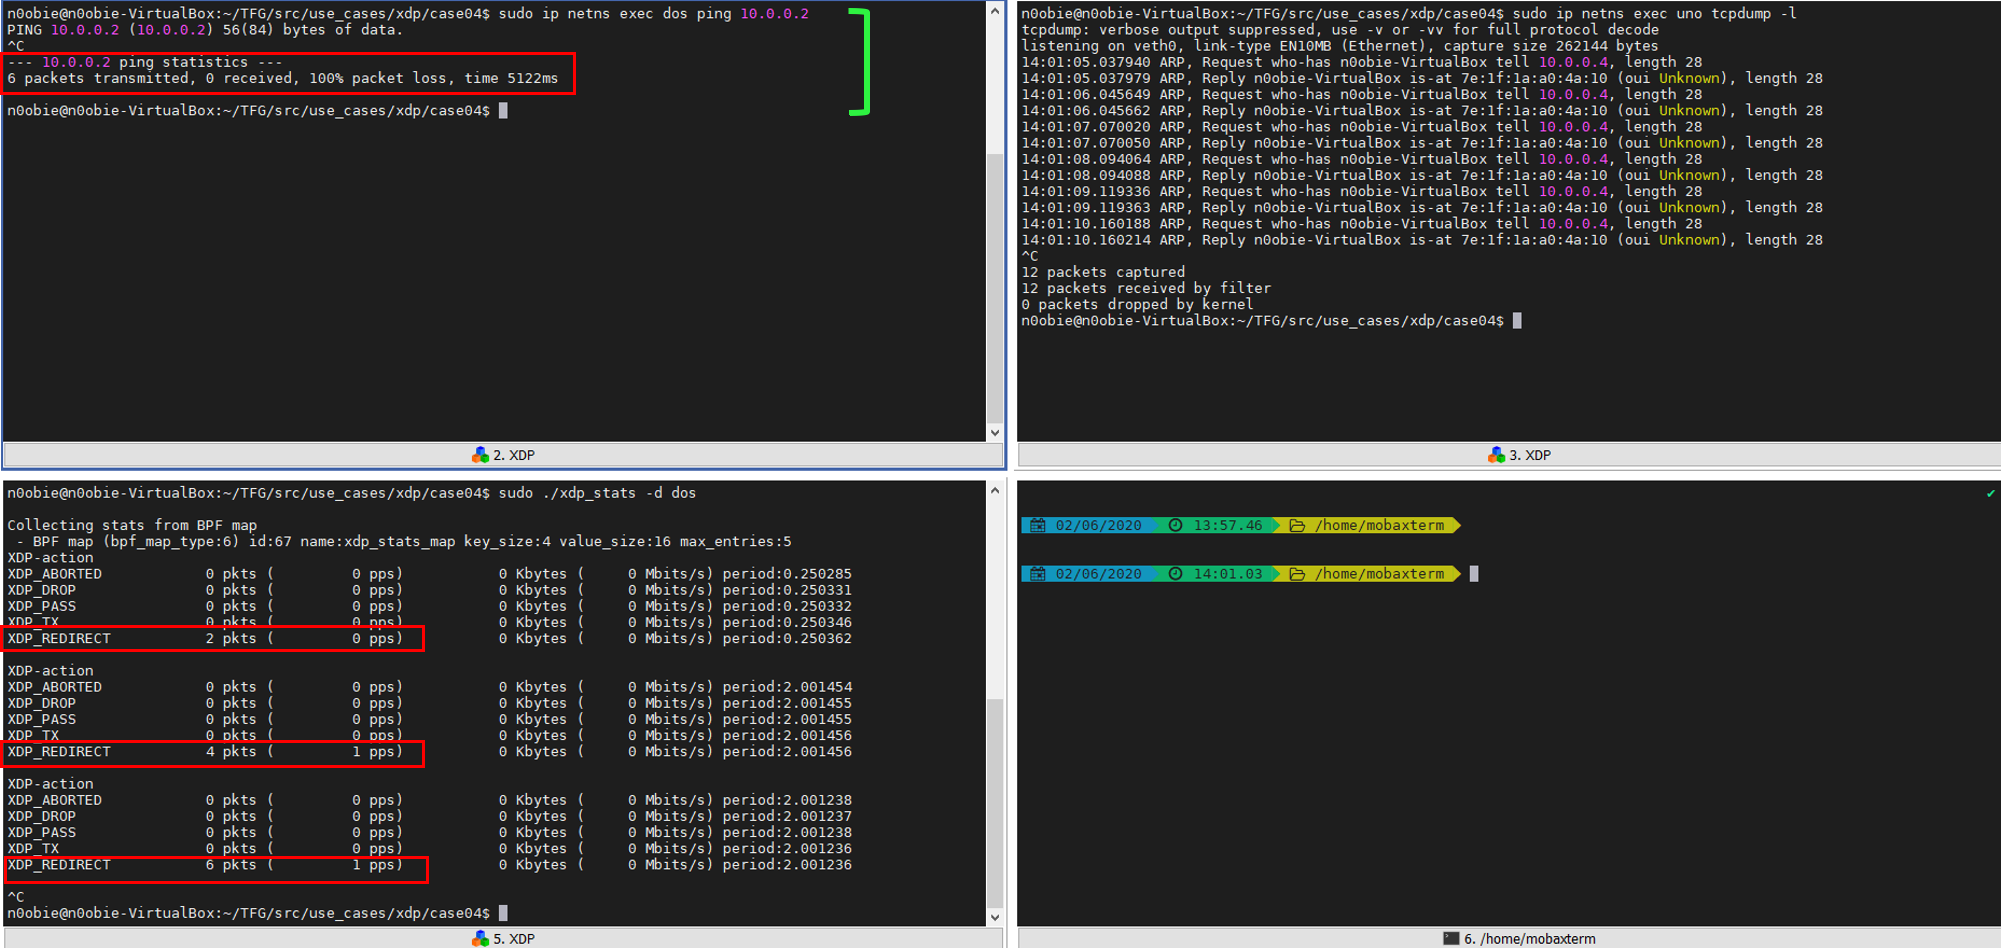
\includegraphics[width=15.5cm]{archivos/img/dev/xdp/case04/demo_case04_hard_1_edited.png}
    \caption{Comprobación de funcionamiento Hardcoded forwarding del Case04 - XDP}
    \label{fig:case04_xdp_ether_func1_b}
\end{figure}

Como se puede apreciar en la figura \ref{fig:case04_xdp_ether_func1_b}, el ping \fcolorbox{black}{green}{\rule{0pt}{2.5pt}\rule{2.5pt}{0pt}}\hspace{1mm} no llega a completarse. Esto se debe a que al implementar una comunicación unidireccional, el ping se queda bloqueado en la resolución ARP. Se puede corroborar este funcionamiento atendiendo a los códigos de retorno \gls{xdp}, \texttt{XDP\_REDIRECT}, como van en aumento debido a los reenvíos de los paquetes ARP-Request de una interfaz a la otra y por la escucha de tcpdump en la terminal superior derecha. 
%%%%%%%%%%%%%%%%%%%%%%%%%%%%%%%%%%%%%%%%%%%%%%%%%%%%%%%%%%%%%%%%%%%%%%%%%%%%%%%%%%%%

\subsubsection{Semi-Hardcoded forwarding (BPF maps)}

La segunda forma de implementar el forwarding se denominará Semi-Hardcoded forwarding, ya que la información irá hardcodeada, pero no en el propio programa \gls{xdp}, sino, en los mapas \gls{bpf}. El escenario levantado se puede apreciar en la figura \ref{fig:case04_xdp_ether_scenario2}, está compuesto de dos \textit{Network Namespace} (\texttt{uno} y \texttt{dos}), y de dos pares de \gls{veth}s (\texttt{veth0} -- \texttt{uno} y \texttt{veth0} -- \texttt{dos}) las cuales se utilizarán para comunicar las dos \textit{Network Namespaces} entre sí, a través del la \textit{Network Namespace} por defecto. En este caso el forwarding se hará desde la interfaz \texttt{dos} hacia la interfaz \texttt{uno} y viceversa, por lo que la comunicación será bidireccional.

% figura escenario
\begin{figure}[ht]
    \centering
    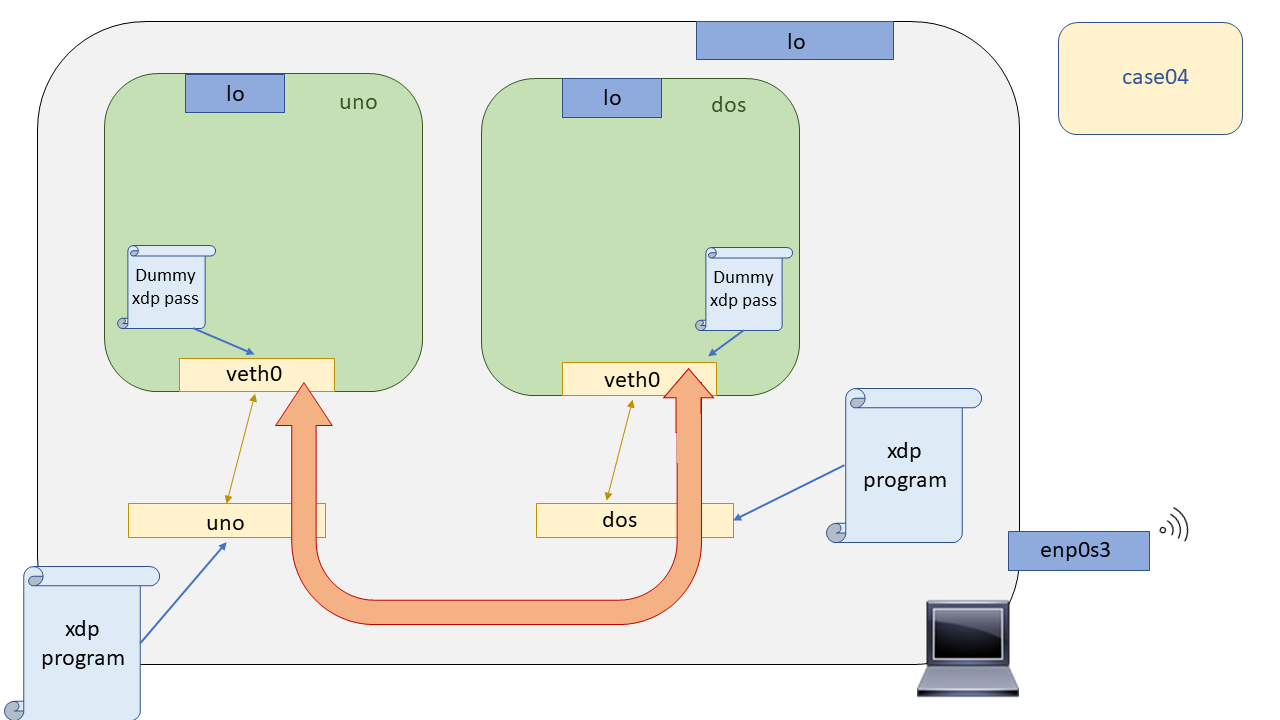
\includegraphics[width=14cm]{archivos/img/dev/xdp/case04/scenario_02.png}
    \caption{Escenario cableado Semi-Hardcoded forwarding del Case04 - XDP}
    \label{fig:case04_xdp_ether_scenario2}
\end{figure}

\vspace{1cm}
\textbf{Carga del programa XDP}\\
\par
Esta manera de hacer el forwarding no requiere de hardcodear datos en el propio programa \gls{xdp} que irá al Kernel, si no, que se usarán los mapas \gls{bpf} como medio para guardar datos de forwarding como son las \textit{ifindex} y las MAC destino desde espacio de usuario. De esta forma, posteriormente el programa anclado en el Kernel sea capaz de leer los mapas, obtener la información de forwarding y realizarlo en base a la información percibida de los mapas \gls{bpf}.\\
\par

De nuevo, y como en este caso la comunicación será bidireccional se debe anclar dos \textit{dummy program} en los dos extremos donde van a llegar los paquetes, si no se está al tanto de esta limitación vuelva a la subsección (\ref{xdp_ether_case04_hard}) donde se menciona la limitación.\\
\par

Es importante señalar que los programas anclados previamente deben ser retirados, por lo que una opción sería hacer un \textit{clean} del escenario haciendo uso del script dado ( \texttt{sudo ./runenv.sh -c}) y empezar de nuevo.\\
\par
\begin{lstlisting}[language= bash, style=Consola, caption={Carga del programa XDP Semi-Hardcoded forwarding - Case04},label=code:case04_xdp_ether_load2]
    # Entramos en cada Network Namespace y anclamos los "dummy programs"
    sudo ip netns exec uno ./xdp_loader -d veth0 -F --progsec xdp_pass
    sudo ip netns exec dos ./xdp_loader -d veth0 -F --progsec xdp_pass
    
    # Anclamos el programa XDP en cada interfaz para conseguir un comunicación bidireccional 
    sudo ./xdp_loader -d uno -F --progsec xdp_case04_map
    sudo ./xdp_loader -d dos -F --progsec xdp_case04_map
    
    # Almacenamos la información necesaria para realizar el forwarding 
    src="uno"
    dest="dos"
    src_mac=$(sudo ip netns exec $src cat /sys/class/net/veth0/address)
    dest_mac=$(sudo ip netns exec $dest cat /sys/class/net/veth0/address)
     
    # Populamos los mapas BPF con la información útil para llevar a cabo el forwarding en ambas direcciones
    ./prog_user -d $src -r $dest --src-mac $src_mac --dest-mac $dest_mac
    ./prog_user -d $dest -r $src --src-mac $dest_mac --dest-mac $src_mac
\end{lstlisting}


\vspace{1cm}
\textbf{Comprobación del funcionamiento}\\
\par
La comprobación de funcionamiento de este programa puede ser llevada a cabo desde un extremo u otro debido a que, si todo funciona correctamente, existirá una comunicación bidireccional. Por lo que, en este caso se harán las pruebas desde la \textit{Network namespace} \texttt{uno} hacia la \texttt{dos}.\\
\par
Como se puede apreciar en la figura \ref{fig:case04_xdp_ether_func2}, existe una comunicación bidireccional ya que el ping \fcolorbox{black}{orange}{\rule{0pt}{2.5pt}\rule{2.5pt}{0pt}}\hspace{1mm} se ejecuta con normalidad. Además, en la subfigura \ref{fig:case04_xdp_ether_func2_stats} se puede ver como los códigos de retorno \gls{xdp} de forwarding van aumentando, por lo que el programa \gls{xdp} está funcionando según lo previsto.

\begin{figure}[h]
    \centering
    \begin{subfigure}[b]{\textwidth}
    	\centering
        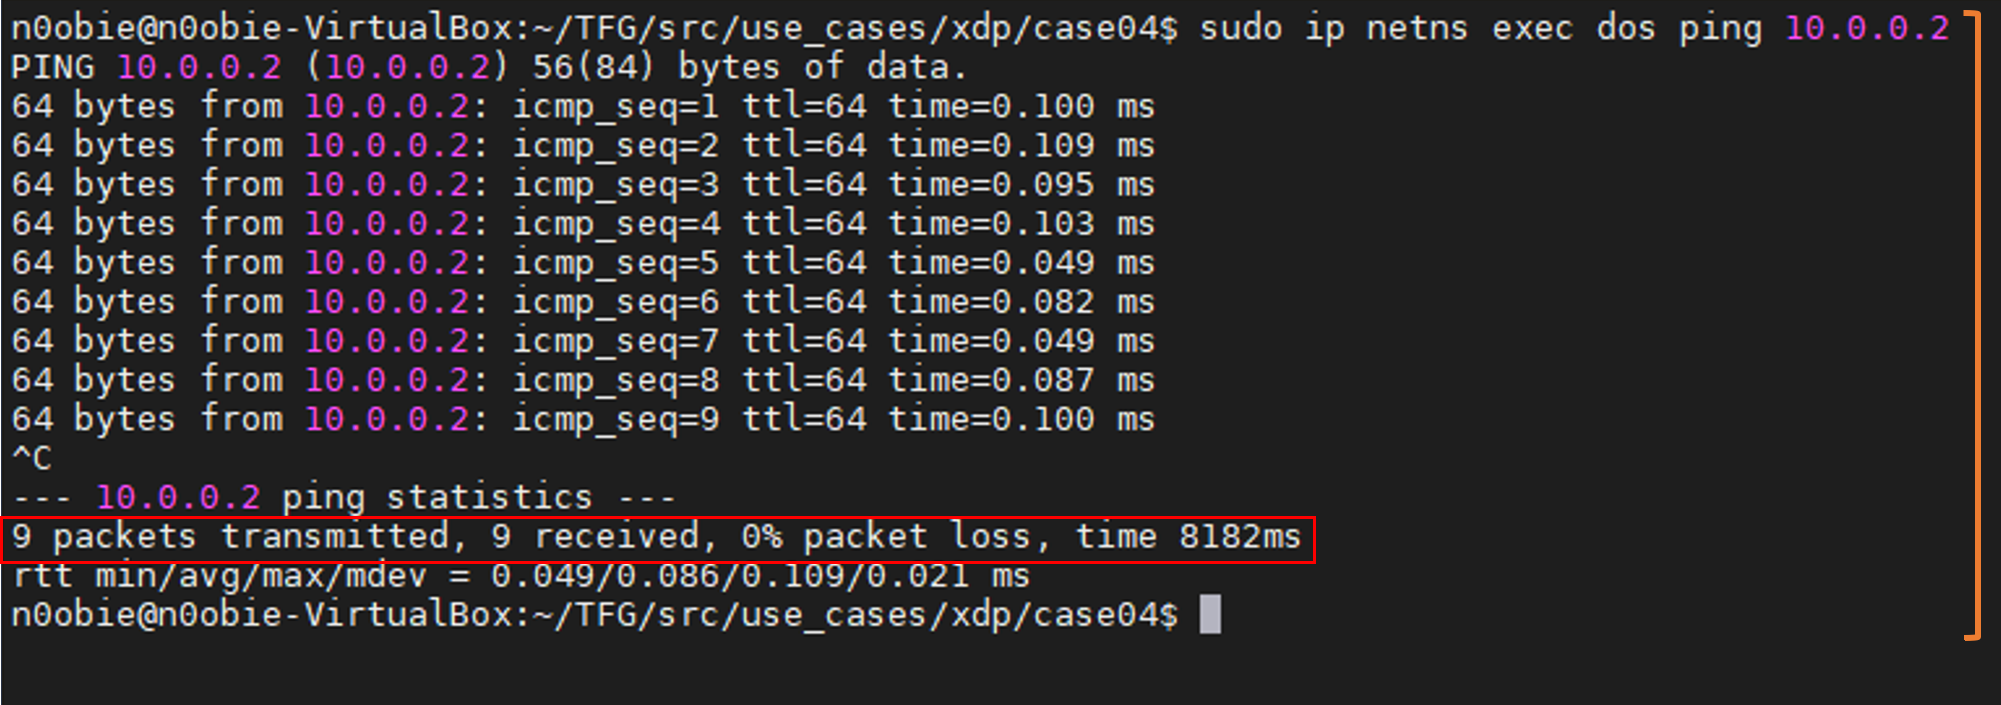
\includegraphics[width=11cm]{archivos/img/dev/xdp/case04/demo_case04_semihard_2_edited.png}
        \caption{Ejecución de ping hacia la interfaz con el programa XDP}
        \label{fig:case04_xdp_ether_func2_ping}
    \end{subfigure}
    \par\bigskip
    \begin{subfigure}[b]{\textwidth}
    	\centering
        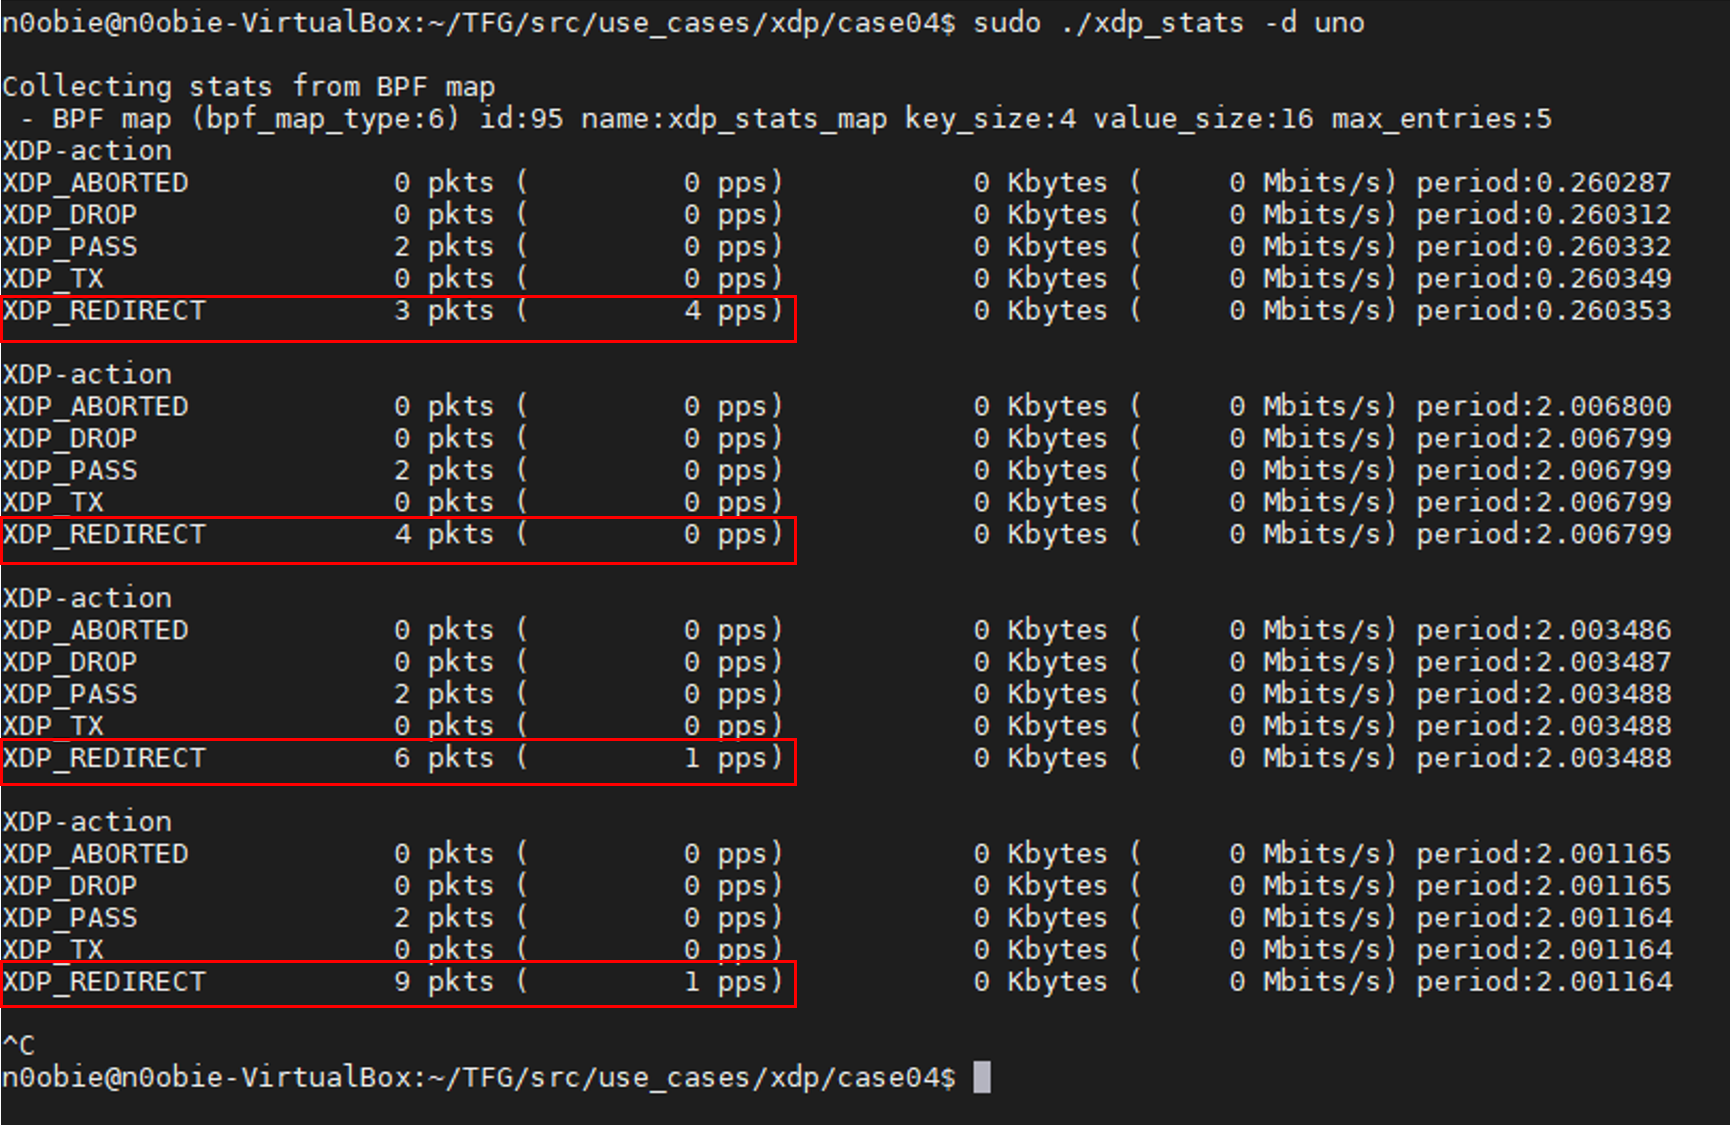
\includegraphics[width=14cm]{archivos/img/dev/xdp/case04/demo_case04_semihard_3_edited.png}
        \caption{Estadísticas de los códigos de retorno XDP}
        \label{fig:case04_xdp_ether_func2_stats}
    \end{subfigure}
    \caption{Comprobación de funcionamiento Semi-Hardcoded forwarding del Case04 - XDP}
    \label{fig:case04_xdp_ether_func2}
\end{figure}

% \todo{Cambiar este bloque de código por una imagen ya que es un resultado}
% \begin{lstlisting}[language= bash, style=Consola, caption={Comprobación del funcionamiento Semi-Hardcoded forwarding - Case04},label=code:case04_xdp_ether_func2]
%     # Hacemos un ping desde el interior de la Network namespace "uno" hacia la veth0 de la Network namespace "dos"
%     ping  {IP_veth_dos} [ y viceversa..]
    
%     # Comprobamos con el recolector de estadísticas que se están produciendo XDP_REDIRECT
%     sudo ./xdp_stats -d uno
    
%     ó
    
%     sudo ./xdp_stats -d dos
% \end{lstlisting}



%%%%%%%%%%%%%%%%%%%%%%%%%%%%%%%%%%%%%%%%%%%%%%%%%%%%%%%%%%%%%%%%%%%%%%%%%%%%%%%%%%%%
\subsubsection{Forwarding auto (Kernel FIBs)}

La tercera forma de hacer forwarding hace referencia al forwarding automático, esto es debido a que no habrá ningún tipo de información de forwarding hardcodeada en el programa \gls{xdp}, la información se obtendrá del propio \textit{stack} de red trabajando de forma cooperativa con éste. El escenario sobre el cual se trabajará será el mismo que el anterior por lo que únicamente es necesario preocuparse de limpiar el escenario de los programas \gls{xdp} anteriormente anclados a cada interfaz para que no interfieran con los nuevos programas \gls{xdp} que se van anclar.\\
\par
En este caso, se va a ir un paso más allá y el forwarding será automático, es decir, no se hardcodeará ningún tipo de información para hacer el forwarding a los paquetes. Pero, entonces: ¿cómo se sabrá a dónde hay que mandar los paquetes? Esta información se conseguirá del \textit{stack} de red del Kernel de Linux el cual tiene una FIB (\textit{Forwarding Information Base}) con reglas muy útiles las cuales se pueden sacar partido. \\
\par
Por lo que, se realizará una consulta a la FIB con el \textit{helper} \texttt{bpf\_fib\_lookup()} para obtener información de forwarding desde el propio \textit{stack} de red, este es un claro ejemplo donde la cooperación con el \textit{stack} de red hace que el programa \gls{xdp} sea más robusto e independiente del espacio de usuario.

% figura escenario
\begin{figure}[ht]
    \centering
    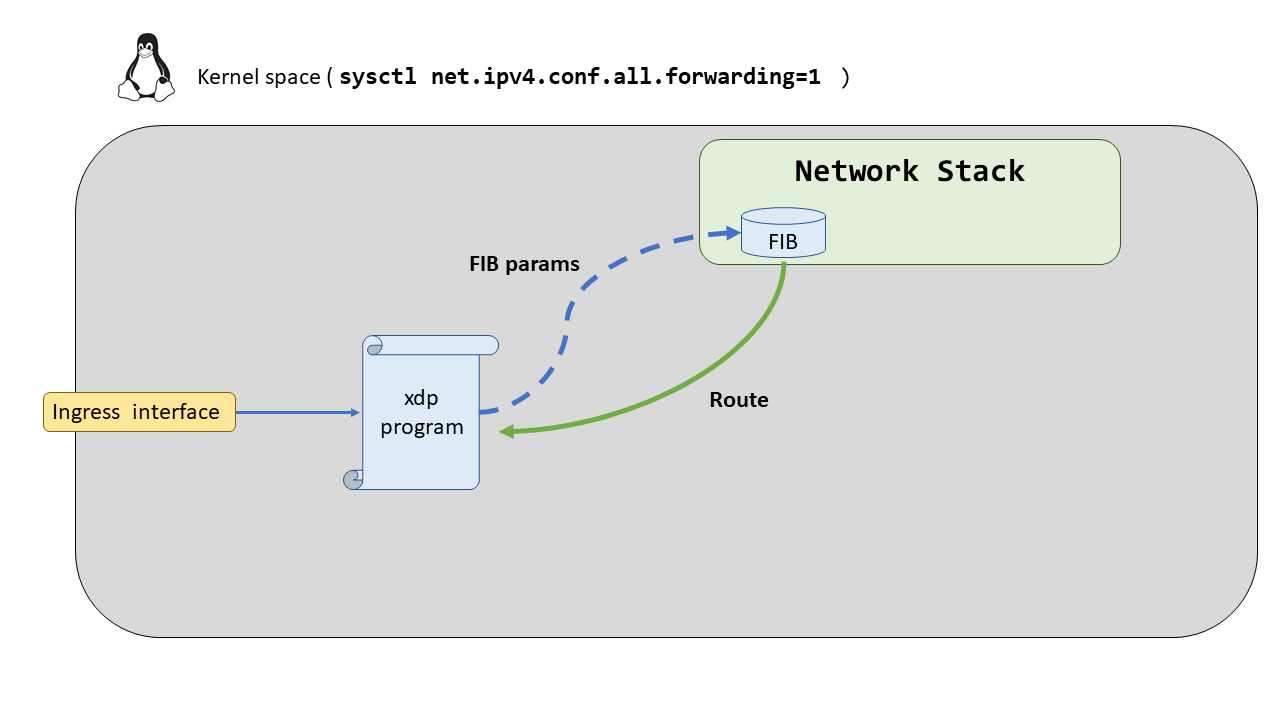
\includegraphics[width=16cm]{archivos/img/dev/xdp/case04/scenario_03.png}
    \caption{Escenario cableado Forwarding auto del Case04 - XDP}
    \label{fig:case04_xdp_ether_scenario3}
\end{figure}
\newpage
\vspace{1cm}
\textbf{Carga del programa XDP}\\
\par
Para la carga del programa \gls{xdp} se deberá primero habilitar el forwarding en nuestro Kernel, acto seguido se anclarán los \textit{dummy program} y por último, se anclarán anclar los programas \gls{xdp} en ambas interfaces tanto \texttt{uno} como \texttt{dos} para conseguir que la comunicación sea bidireccional.
\vspace{0.5cm}

\begin{lstlisting}[language= bash, style=Consola, caption={Carga del programa XDP Forwarding auto - Case04},label=code:case04_xdp_ether_load3]
    # Habilitamos el forwarding 
    sudo sysctl net.ipv4.conf.all.forwarding=1
    
    # Anclamos los programas XDP a cada interfaz 
    sudo ./xdp_loader -d uno -F --progsec xdp_case04_fib
    sudo ./xdp_loader -d dos -F --progsec xdp_case04_fib
    
    # Ahora añadimos a cada interfaz destino su "dummy program"
    sudo ip netns exec uno ./xdp_loader -d veth0 -F --progsec xdp_pass
    sudo ip netns exec dos ./xdp_loader -d veth0 -F --progsec xdp_pass
    
    # Habilitamos los ifindex 
    sudo ./prog_user -d uno
    sudo ./prog_user -d dos
\end{lstlisting}

\vspace{1cm}

\textbf{Comprobación del funcionamiento}\\
\par
La comprobación de funcionamiento de este programa puede ser llevada a cabo desde un extremo u otro debido a que, si todo funciona correctamente, existirá una comunicación bidireccional y completamente automática ya que no ha almacenado ningún tipo de información en los programas anclados. Por lo que, se harán las pruebas desde la \textit{Network namespace} \texttt{uno} hacia la \texttt{dos}. Como se puede apreciar en la figura \ref{fig:case04_xdp_ether_func3}, atendiendo al funcionamiento del ping \fcolorbox{black}{yellow}{\rule{0pt}{2.5pt}\rule{2.5pt}{0pt}}\hspace{1mm}, hay una perfecta comunicación entre ambas \textit{Network namespaces}, por lo que el programa está tomando correctamente las rutas de la FIB. \\

% \todo{Cambiar este bloque de código por una imagen ya que es un resultado}
\begin{lstlisting}[language= bash, style=Consola, caption={Comprobación del funcionamiento Forwarding auto - Case04},label=code:case04_xdp_ether_func3]
    # Hacemos un ping desde el interior de la Network namespace "uno" hacia la veth0 de la Network namespace "dos"
    ping  {IP_veth_dos} [ y viceversa..]
    
    # Comprobamos con el recolector de estadísticas que se están produciendo XDP_REDIRECT
    sudo ./xdp_stats -d uno

\end{lstlisting}

\newpage

\begin{figure}[h]
    \centering
    \begin{subfigure}[b]{\textwidth}
    	\centering
        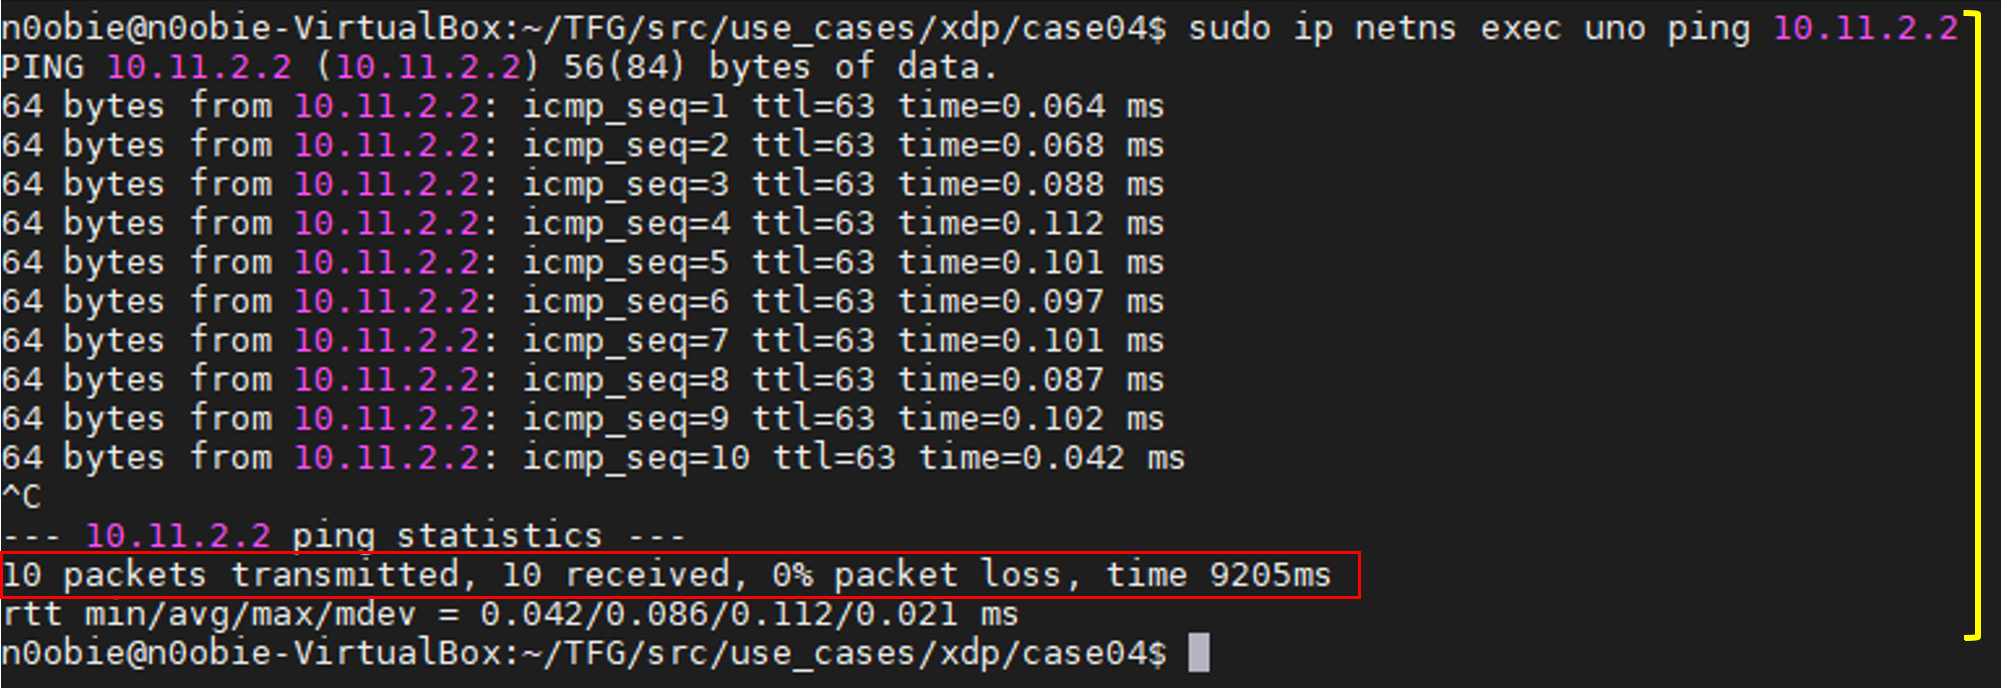
\includegraphics[width=13cm]{archivos/img/dev/xdp/case04/demo_case04_auto_2_edited.png}
        \caption{Ejecución de ping hacia la interfaz con el programa XDP}
        \label{fig:case04_xdp_ether_func3_ping}
    \end{subfigure}
    \par\bigskip
    \begin{subfigure}[b]{\textwidth}
    	\centering
        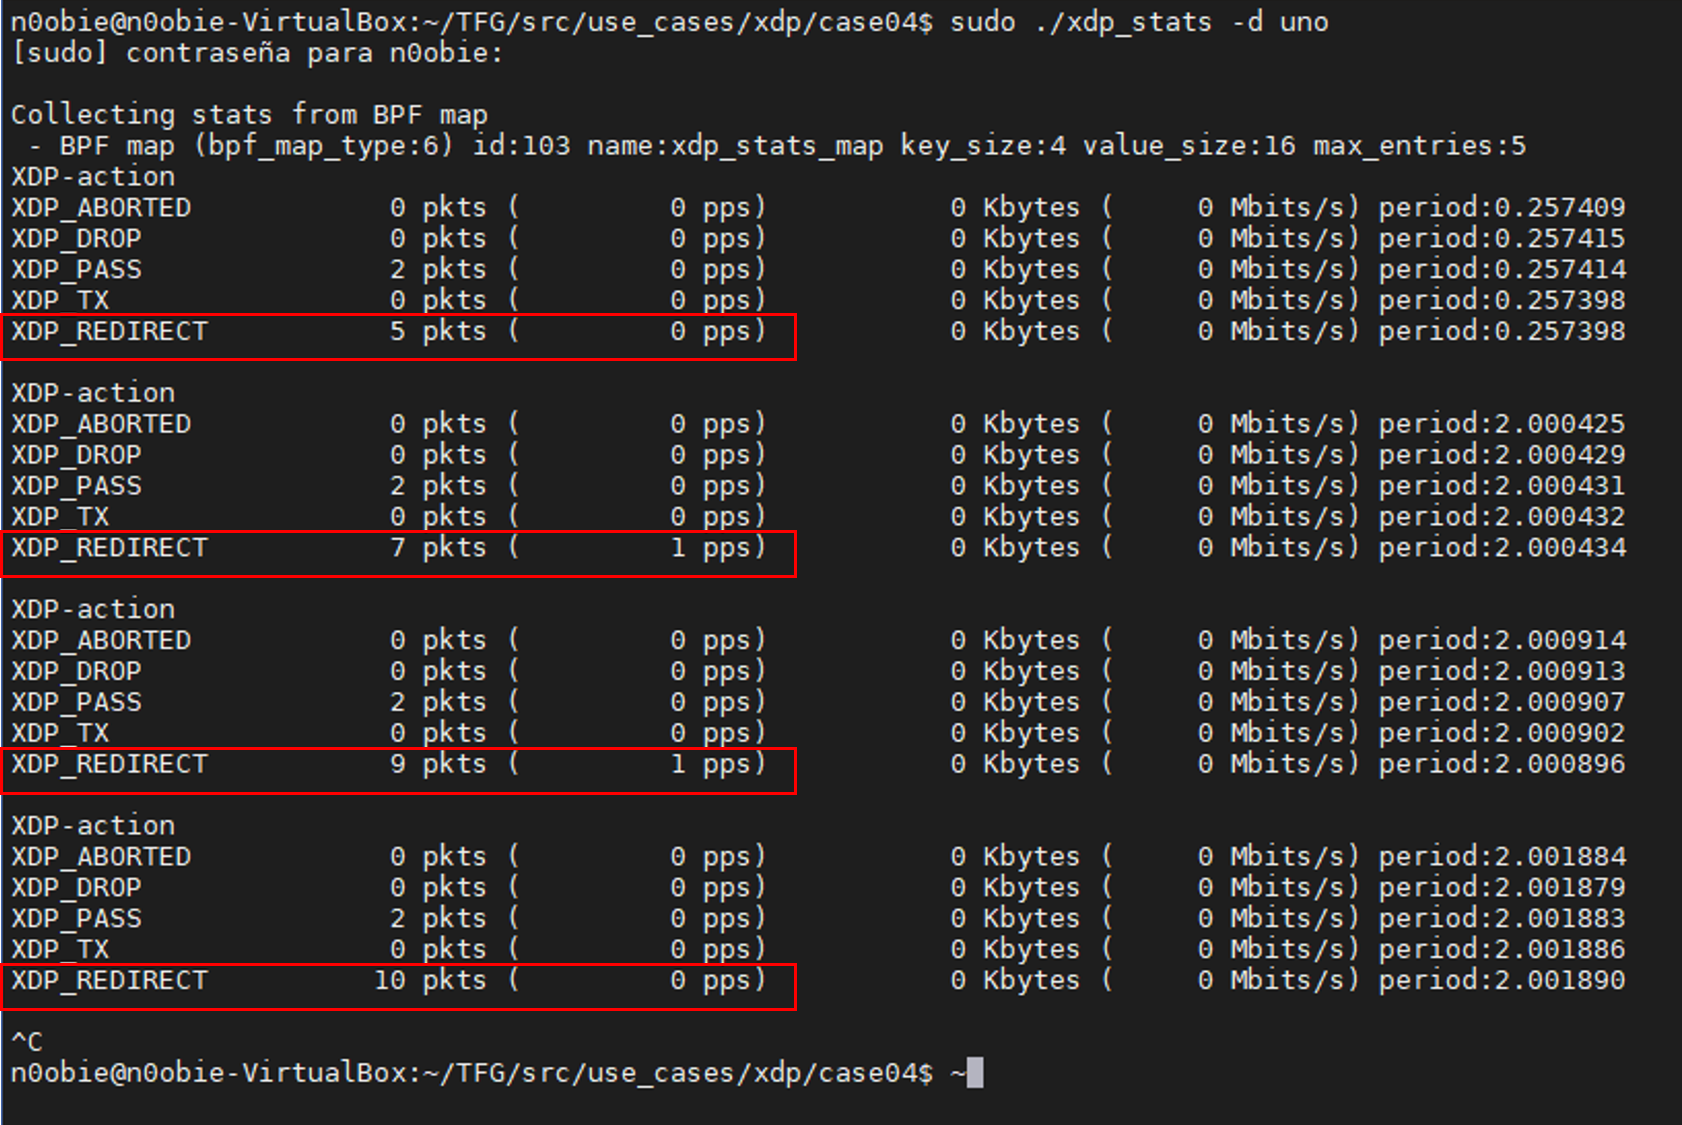
\includegraphics[width=14cm]{archivos/img/dev/xdp/case04/demo_case04_auto_3_edited.png}
        \caption{Estadísticas de los códigos de retorno XDP}
        \label{fig:case04_xdp_ether_func3_stats}
    \end{subfigure}
    \caption{Comprobación de funcionamiento Forwarding auto del Case04 - XDP}
    \label{fig:case04_xdp_ether_func3}
\end{figure}